\documentclass[thmcnt=section, color=cyan, 12pt]{my-elegantbook}

% index page
\usepackage{imakeidx}
\makeindex[columns=2, intoc, options=-s index_style.ist]

% title and author
\title{Complex Analysis}
\author{Isaac FEI}

% reference file
\addbibresource{complex-analysis.bib} 

% image of the book cover
\cover{cover}

\begin{document}

% Print title and cover page
\maketitle

%--------
% preface
%--------

\frontmatter
\chapter*{Preface}

This book mainly follows the structure of \cite{steinComplexAnalysis2003}.

%------------------------------

% Print table of contents
\tableofcontents
\mainmatter

%-------------------------------
% main document starts from here
%-------------------------------

%==============================

\chapter{Point-Set Topology}

%------------------------------

\section{Preimages}

Let $f: X \to Y$ be a function between two sets. The \textbf{preimage}\index{preimage} of a subset $S \subseteq Y$ under $f$,
written $f^{-1}(S)$, is defined by
\begin{align*}
    f^{-1}(S) := \{x \in X \mid f(x) \in S\}
\end{align*}
In other words,
\begin{align*}
    x \in f^{-1}(S) \iff f(x) \in S
\end{align*}

%==============================

\chapter{Cauchy's Theorem and Its Applications}

%------------------------------

\section{Goursat's Theorem}

\begin{theorem}[Goursat's Theorem] \label{thm:4}
    Let $\Omega \subseteq \C$ be an open set and $T \subseteq \Omega$ a triangle whose interior is also contained in $\Omega$.
    If $f$ is holomorphic in $\Omega$, then
    \begin{align*}
        \int_{T} f(z) \dif z = 0
    \end{align*}
\end{theorem}

We could state and prove Goursat's Theorem
considering the counter integral along a rectangle.
But we will see in Corollary~\ref{cor:1}
that the rectangle version is an immediate corollary of this triangle version
since we can divide a rectangle into two triangles.

\begin{proof}
    % TODO
\end{proof}

\begin{corollary} \label{cor:1}
    If $f$ is holomorphic in an open set $\Omega$
    containing a rectangle $R$ and its interior, then
    \begin{align*}
        \int_{R} f(z) \dif z = 0
    \end{align*}
\end{corollary}

%------------------------------

\section{Local Existence of Primitives and Cauchy's Theorem in a Disk}

\begin{theorem}
    If $f$ is holomorphic in an open disk $D \subseteq \C$, then $f$ has a primitive there.
\end{theorem}

\begin{proof}
    Without loss of generality, we may assume the disk $D$ is centered at the origin.
    If it is centered at $z_0$,
    we can translate the disk to the origin and define $f(z) = f(z + z_0)$.
    Then we find a primitive for $f$, say $F$.
    The primitive for $f$ is then given by $F(z) = F(z - z_0)$.

    Assume $D$ is centered at the origin,
    we are going to construct a primitive $F$ for $f$ in $D$
    using a contour integral.
    For any point $z \in D$,
    curve $\gamma_z$ is taken to be the horizontal line segment
    from $0$ to $\RE z$
    followed by the vertical segment from $\RE z$ to $z$.
    Note that $\gamma_z$ is indeed contained in $D$.
    Let function $F$ be defined by
    \begin{align*}
        F(z) = \int_{\gamma_z} f(w) \dif w
    \end{align*}
    We will show $F$ is indeed a primitive for $f$ in $D$.
    Hence, we need to estimate the quotient $\frac{F(z+h) - F(z)}{h}$ when $h \to 0$.

    This invites us to consider the contour integral of $f$ along curve $\gamma_{z_h} - \gamma_z$. As illustrated in Figure~\ref{fig:1},
    by adding a rectangle and a triangle without change the value of the contour integral
    due to Theorem~\ref{thm:4} and Corollary~\ref{cor:1}, one may verify that
    \begin{align}
        F(z+h) - F(z)
        = \int_{\gamma_{z+h} - \gamma_z} f(w) \dif w
        = \int_\eta f(w) \dif w
        \label{eq:6}
    \end{align}
    where $\eta$ is the line segment from $z$ to $z+h$.

    \begin{figure}[H]
        \centering
        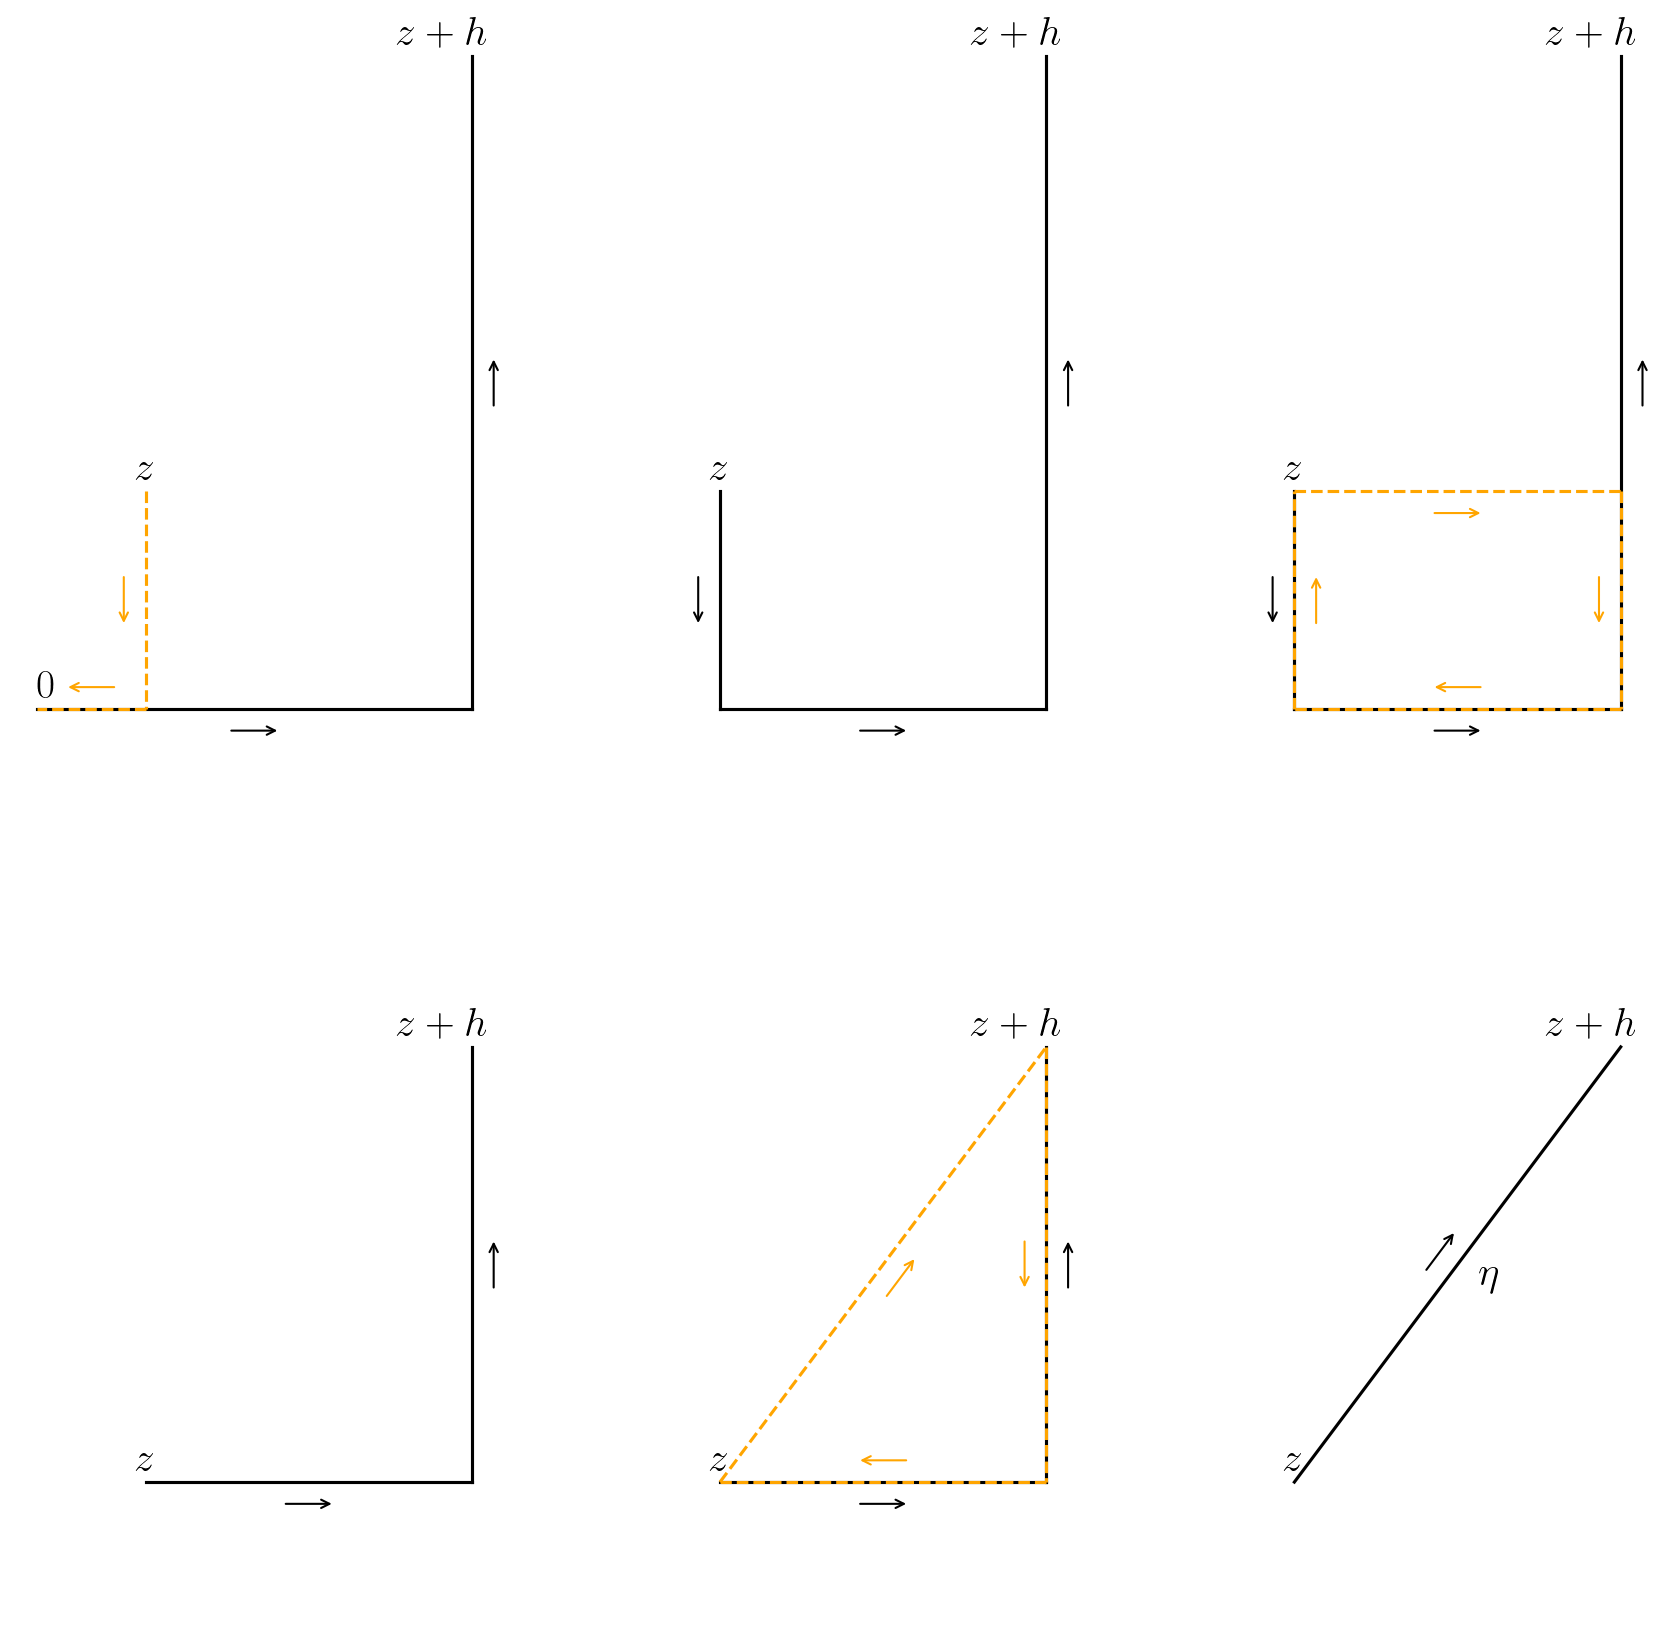
\includegraphics[scale=0.3]{figures/adding-a-rectangle-and-a-triangle.png}
        \caption{Construction of curve $\eta$ by adding a rectangle and a triangle to the curve $\gamma_{z+h} - \gamma_z$.}
        \label{fig:1}
    \end{figure}

    Now, we are going to estimate $f(w)$ about the point $z$. Because $f$ is continuous, we can write
    \begin{align*}
        f(w) = f(z) + \psi(w), \quad w \in D \setminus \{z\}
    \end{align*}
    where $\psi(w)$ is continuous and
    \begin{align*}
        \lim_{w \to z} \psi(w) = 0
    \end{align*}

    \begin{note}
        Estimating $f(w)$ about $z$ using the derivative of $f$ at $z$,
        like what we did in the proof of Theorem~\ref{thm:4}, may be an overkill.
        It suffices to estimate $f(w)$ by exploiting the continuity of $f$.
        We have already used the fact that $f$ is holomorphic to construct
        the curve $\eta$ by applying the Goursat's theorem.
    \end{note}

    It then follows that
    \begin{align}
        \int_\eta f(w) \dif w
         & = \int_\eta f(z) + \psi(w) \dif w                    \nonumber \\
         & = f(z) \int_\eta 1 \dif w + \int_\eta \psi(w) \dif w \nonumber \\
         & = f(z) h + \int_\eta \psi(w) \dif w
        \label{eq:7}
    \end{align}
    Combining \eqref{eq:6} and \eqref{eq:7}, we have
    \begin{align}
        \abs{\frac{F(z+h) - F(z)}{h} - f(z)}
         & = \frac{1}{\abs{h}} \abs{\int_\eta \psi(w) \dif w}            \nonumber  \\
         & \text{Apply the ML inequality}                                 \nonumber \\
         & \leq \frac{1}{\abs{h}} \max_{w \in \eta} \abs{\psi(w)} \abs{h} \nonumber \\
         & = \max_{w \in \eta} \abs{\psi(w)}
        \label{eq:8}
    \end{align}
    As $h \to 0$, we have $w \to z$ and hence $\psi(w) \to 0$.
    Therefore, the limit of the right-hand side of \eqref{eq:8}
    is $0$ as $h \to 0$.
    This proves $F^\prime(z) = f(z)$.
\end{proof}

%------------------------------

\section{Cauchy's Integral Formula}

\begin{theorem} \label{thm:1}
    Suppose $f$ is holomorphic in an open set $\Omega$, and $D$ is an open disk
    centered at $z_0$ whose closure is contained in $\Omega$. Then $f$ has a power
    series expansion at $z_0$ in the form
    \begin{align}
        f(z) = \sum_{n=0}^\infty \frac{f^{(n)}(z_0)}{n!}  (z - z_0)^n \quad \forall z \in D
        \label{eq:1}
    \end{align}
\end{theorem}

\begin{theorem}[Liouville's Theorem] \label{thm:2}
    % TODO
\end{theorem}

\begin{theorem}[Fundamental Theorem of Algebra] \label{thm:3}
    Every polynomial with degree greater than $0$ with complex coefficients has a
    root in $\C$.
\end{theorem}

\begin{proof}
    Let polynomial $p(z)$ be given by
    \begin{align*}
        p(z) = a_n z^n + \cdots a_1 z + a_0
    \end{align*}
    where $n \geq 1$ and $a_n \neq 0$.
    We shall prove by contradiction.
    Assume $p(z)$ has no roots in $\C$. Then the reciprocal $1 / p(z)$ is defined on the entire
    complex plane.
    Moreover, the derivative of $1 / p(z)$ clearly exists everywhere.
    Therefore, $1 / p(z)$ is entire.
    We will use Liouville's theorem to establish a contradiction.
    To do so, we are going to show $1 / p(z)$ is bounded.

    We have
    \begin{align*}
        \frac{p(z)}{z^n} = a_n + \frac{a_{n-1}}{z} + \cdots + \frac{a_1}{z^{n-1}} + \frac{a_0}{z^n}
    \end{align*}
    Note that when $\abs{z} \to \infty$, the modulus of the quotient $p(z) / z^n$ will
    tend to $\abs{a_n}$.
    This implies that there exists $R > 0$ such that
    \begin{align}
        \abs{\frac{p(z)}{z^n}} > \frac{\abs{a_n}}{2}
        \label{eq:2}
    \end{align}
    whenever $\abs{z} > R$. Rearranging \eqref{eq:2}, we have
    \begin{align*}
        \abs{\frac{1}{p(z)}} < \frac{2}{\abs{a_n}} \cdot \frac{1}{\abs{z}^n} < \frac{2}{\abs{a_n} R^n} \quad \text{if } \abs{z} > R
    \end{align*}
    The above inequality shows $1 / p(z)$ is bounded outside the disk $D$ centered
    at $0$ with radius $R$.

    For points inside the closed disk $\overline{D}$, since function $\abs{1 / p(z)}$ is
    continuous and $\overline{D}$ is compact, $\abs{1 / p(z)}$ attains its maximum $M$ on $\overline{D}$.

    Therefore, we see that $1 / p(z)$ is indeed bounded on entire complex plane $\C$.
    By Liouville's theorem \ref{thm:2}, $1 / p(z)$ is constant, which leads to a
    contradiction since polynomials with degree greater than $0$ are non-constant.


    \begin{note}
        The last assertion that polynomials with degree greater than $0$ are
        non-constant seem evident. But the reader should still prove it. See Proposition~\ref{pro:1}.
        And the proof is not that trivial.
    \end{note}
\end{proof}

\begin{proposition} \label{pro:1}
    Polynomials with degree greater than $0$ are non-constant.
\end{proposition}

Now, we have proved polynomial $p(z)$ must have one root. Using mathematical
induction we can show that it actually has $n$ roots, and can be factorized as
\begin{align*}
    p(z) = a_n (z^n - z_1) (z^n - z_2) \cdots (z^n - z_n)
\end{align*}

\begin{corollary}
    Every polynomial $p(z) = a_n z^n + \cdots + a_1 z + a_0$ of degree $n \geq 1$ with
    complex coefficients has exactly $n$ roots in $\C$. If these $n$ roots are
    denoted by $z_1, \ldots, z_n$, then $p(z)$ can be factorized as
    \begin{align*}
        p(z) = a_n (z^n - z_1) (z^n - z_2) \cdots (z^n - z_n)
    \end{align*}
\end{corollary}

\begin{proof}
    We shall prove by induction.

    \noindent\textbf{Base Case:} Suppose $n = 1$, then $p(z) = a_1 z + a_0$ ($a_1 \neq 0$). Setting $p(z) = 0$, we solve that $z = -a_0 / a_1$. Therefore, $z_1 = -a_0 / a_1$ is the only root of $p(z)$, and we can write $p(z) = a_1(z - z_1)$.

    \noindent\textbf{Inductive Step:} Assume this corollary holds for $n = k$, we need to show that it also holds for $n = k + 1$.
    By the Fundamental Theorem of Algebra \ref{thm:3}, there exists one root $z_1$ for $p(z)$.
    We want to show that $p(z)$ has a factor $(z - z_1)$.
    Let $\tilde{p}(z) = p(z + z_1)$.
    Note that $\tilde{p}(z)$ is also a polynomial of degree $k + 1$.
    Write
    \begin{align}
        \tilde{p}(z) = b_{k+1} z^{k+1} + \cdots + b_1 z + b_0
        \label{eq:3}
    \end{align}
    Because $z_1$ is a root of $p(z)$, we have $\tilde{p}(0) = p(z_1) = 0$. Substituting $z=0$ into \eqref{eq:3} yields $b_0 = 0$.
    Therefore, we can write
    \begin{align*}
        \tilde{p}(z) = z (b_{k+1} z^{k} + \cdots b_2 z + b_1)
    \end{align*}
    Then, we recover the expression of $p(z)$ from $\tilde{p}(z)$.
    Note that $p(z) = \tilde{p}(z - z_1)$.
    Hence,
    \begin{align*}
        p(z) = (z - z_1) \underbrace{(b_{k+1} z^{k} + \cdots b_2 z + b_1)}_{\text{a polynomial of degree $k$}}
        = (z - z_1) q(z)
    \end{align*}
    Now, we may apply the induction hypothesis on $q(z)$.
    We have
    \begin{align*}
        p(z) & = (z - z_1) [c (z - z_2) \cdots (z - z_{k+1})] \\
             & = c (z - z_1) \cdots (z - z_{k+1})
    \end{align*}
    And we realized that $c$ is exactly $a_{k+1}$ since it is the coefficient of $z^{k+1}$.
    Therefore, we have shown
    \begin{align}
        p(z) = a_{k+1} (z - z_1) \cdots (z - z_{k+1})
        \label{eq:4}
    \end{align}
    Equation~\eqref{eq:4} tells us that $z_1, \ldots, z_{k+1}$ are roots of $p(z)$.
    Moreover, $p(z)$ cannot have any other roots. To see this, suppose $w \neq z_j \ \forall j=1, \ldots, k+1$. Then, substituting $z = w$ in \eqref{eq:4}, we see that $p(w) \neq 0$ since each factor is nonzero.
\end{proof}


The next theorem roughly demonstrates that the global behaviour of a holomorphic function is determined by its values on an appropriate small subset.

\begin{theorem}
    If $f$ is a holomorphic function in a connected open set $\Omega$, and vanishes on a sequence of distinct points whose limit is also in $\Omega$, then $f$ is constantly zero in $\Omega$.

    In other words, let $f$ be a holomorphic function in a connected open set $\Omega$.
    Suppose $\{z_n\}_{n \in \Z^+}$ is a sequence of distinct points in $\Omega$, and it converges to $z_0 \in \Omega$. If $f(z_n) = 0$ for all $n$ and $f(z_0) = 0$, then $f(z) = 0$ for all $z \in \Omega$.
\end{theorem}

At a first glance, this result seems magical and almost unrealistic.
How can the value of a function vanishes in the entire set only because it vanishes on a sequence of distinct points?


\begin{proof}
    We will first show that $f$ vanishes in an open disk $D_r(z_0)$ of $z_0$.
    Since $f$ is holomorphic in $\Omega$, it is given by its Taylor series expansion at $z_0$:
    \begin{align*}
        f(z) = \sum_{n=0}^\infty a_n  (z - z_0)^n \quad \forall z \in D_r(z_0)
    \end{align*}
    Assume $f$ is not constantly zero.
    Then we can find the first nonzero coefficient $a_m$ in the expansion.
    Write
    \begin{align}
        f(z) & = a_m(z - z_0)^m + \sum_{k=1}^\infty a_{m+k}  (z - z_0)^{m+k} \nonumber \\
             & = a_m(z - z_0)^m \left[
            1 + \sum_{k=1}^\infty \frac{a_{m+k}}{a_m}  (z - z_0)^{k}
            \right]
        \label{eq:5}
    \end{align}
    Note that the term $\sum_{k=1}^\infty \frac{a_{m+k}}{a_m}  (z - z_0)^{k}$ is a continuous function that vanishes at $z_0$.
    Hence, we may find a sufficiently small neighbourhood $N$ of $z_0$ such that $1 + \sum_{k=1}^\infty \frac{a_{m+k}}{a_m}  (z - z_0)^{k}$ is nonzero in $N$.
    By the given condition, there exists a point $z_j$ in the sequence such that $z_j \neq z_0$ and $z_j \in N$.
    Plugging $z_j$ into \eqref{eq:5}, we have
    \begin{align*}
        0 = f(z_j) = a_m(z_j - z_0)^m \left[
            1 + \sum_{k=1}^\infty \frac{a_{m+k}}{a_m}  (z_j - z_0)^{k}
            \right]
    \end{align*}
    This leads to a contradiction since the right-hand side is nonzero.
    Therefore, $f$ is constantly zero in the disk $D_r(z_0)$.

    Next, we will show that $f$ is zero in the entire set $\Omega$ by exploiting the fact that $\Omega$ is connected.
    Let set $U$ be defined as the interior of the set of all points at which $f$ vanishes, i.e., $U = [f^{-1}(\{0\})]^\circ$
    \begin{note}
        We apply the interior here to enforce that $U$ is open. Now, we will show that it is also closed and hence $U = \Omega$. (Of course, $U \neq \emptyset$.)
    \end{note}

    Note that $U$ is a nonempty open subset of $\Omega$.
    Let $w$ be an accumulation point of $U$.
    Then we can find a sequence $\{w_n\}$ of distinct points in $U$.
    And by the definition of $U$, $f(w_n) = 0 \; \forall n$.
    Applying what we have proved above, we conclude that $f(z) = 0 \; \forall z \in D_{r^\prime} (w)$.
    This shows that $w \in U$.
    Therefore, $U$ contains all its points of accumulation, which means it is also closed.
    Because $\Omega$ is connected and $U$ is a nonempty, both open and closed subset in $\Omega$, it follows that $U = \Omega$.
    Therefore, $f(z) = 0 \; \forall z \in \Omega$.
\end{proof}

%------------------------------


%==============================

% references
\printbibliography[heading=bibintoc, title=References]

%==============================

% print index page
\printindex

\end{document}